%% This is file `BeamerAnimation.tex'
%% Version: 1.0.1
%% Version date: 2018-15-12
%%
%% Copyright (C) 2018 by Luis Paulo Laus, laus@utfpr.edu.br
%%
%% This package can be redistributed and/or modified under the terms
%% of the LaTeX Project Public License distributed from CTAN
%% archives in directory macros/latex/base/lppl.txt; either
%% version 1 of the License, or (at your option) any later version,
%% with `The Package' referring to the software `tikzlibrarycircuits.plc.sfc.code.tex'
%% and its accompanying documentation and `The Copyright Holder' referring to
%% the person Luis Paulo Laus.
%%
%% IMPORTANT NOTICE:
%%
%% For error reports, comments or suggestions in case of UNCHANGED
%% versions send mail to:
%% laus@utfpr.edu.br
%%
%%

\documentclass{beamer}
\usepackage{tikz,units}
\usetikzlibrary{backgrounds, circuits.plc.sfc}

\makeatletter
\newcommand*{\overlaynumber}{\number\beamer@slideinframe}
\makeatother

\tikzset{ % alt and visible (overlay)
  alt/.code args={<#1>#2#3}{%
    \alt<#1>{\pgfkeysalso{#2}}{\pgfkeysalso{#3}}
  },
  visible/.code args={<#1>#2}{%
    \alt<#1>{\pgfkeysalso{#2}}{}
  }
}

\colorlet{LBlue}{blue!20}
\colorlet{LRed}{red!30}

\begin{document}

\begin{frame}{Delta-star motor starter with dead time in SFC: \overlaynumber{}}
\begin{columns}[c]

\column{0.4\textwidth}

\noindent \begin{center}
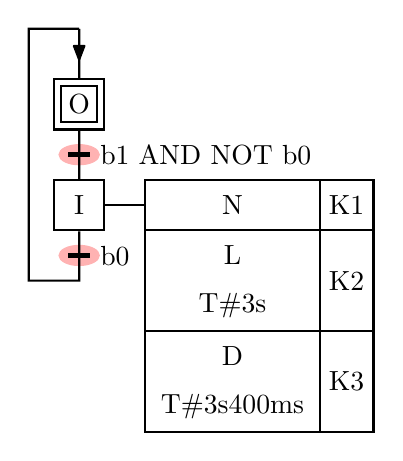
\begin{tikzpicture}[circuit plc sfc,thick,x=2.6\tikzcircuitssizeunit,
  y=1.3\tikzcircuitssizeunit,sfcaqw=9\tikzcircuitssizeunit]
  \draw (0,0)
     to [flow direction={pos=0.95}] ++(0,-1)
     to [sfcstepi={info=O,visible={<1,2,7>{fill=LBlue}}}] ++(0,-4)
     node [sfctransition={info=b1 AND NOT b0},name=t1,visible={<2>{red}}] {}
     to [sfcstep={info=I,visible={<3-6>{fill=LBlue}},
            sfcaction={info=K1,qualifier=N,visible={<3-6>{fill=LBlue}}},
            sfcaction={info=K2,qualifier=L,time=T\#3s,visible={<3>{fill=LBlue}}},
            sfcaction={info=K3,qualifier=D,time=T\#3s400ms,visible={<5-6>{fill=LBlue}}}}] ++(0,-4)
     node [sfctransition={info=b0},name=t2,visible={<6>{red}}]{}
     |- ++(-1,-1) |- (0,0);
  \begin{pgfonlayer}{background}
\visible<2>{
    \draw[fill=LRed,LRed](t1) circle (0.4);
}
\visible<6>{
    \draw[fill=LRed,LRed](t2) circle (0.4);
}
  \end{pgfonlayer}
\end{tikzpicture}
\par\end{center}
\column{0.6\textwidth}
Delta-star with dead time:
\begin{itemize}[<+->]
\item initially, the motor is off
\item b1 is pressed
\item K1 and K2 are activated -- star
\item after $\unit[3]{s}$, K2 is deactivated -- dead time
\item after $\unit[0.4]{s}$, K3 is activated -- delta
\item b0 is pressed
\item motor is off
\end{itemize}
\end{columns}
\noindent \begin{center}
\par\bigskip
Copyright (C) 2018 by Luis Paulo Laus, laus@utfpr.edu.br
\end{center}
\end{frame}
\end{document}